\chapter{Introducción}
\thispagestyle{empty}

\section{Definición del problema}

En la era digital actual, las imágenes faciales han adquirido una relevancia significativa (véase Figura~\ref{fig1} \footnote{Las búsquedas se pueden consultar en el apéndice.}), dado su amplio uso  en aplicaciones multimedia, redes sociales, sistemas de vigilancia y seguridad para la identificación de personas o control de accesos en edificios, así como en investigaciones criminales y forenses para la identificación de sospechosos o la reconstrucción de rostros.
Esta expansión se debe en gran medida al continuo desarrollo tecnológico, que ha mejorado tanto la calidad como la ubicuidad de las fotografías faciales, permitiendo su presencia en una variedad cada vez mayor de contextos y aplicaciones.

\begin{figure}[h]
	\centering
	\includegraphics[scale=0.6]{imagenes/cap1/tabla_facial_images.png}
	\caption[Número de publicaciones de imágenes faciales.]{Número de publicaciones, en Scopus, relacionadas con imágenes faciales en los últimos 45 años.}\label{fig1}
\end{figure}

En este contexto, es importante resaltar el papel que tienen las imágenes faciales en campos como la biometría para la verificación de identidad, así como en la seguridad nacional, donde se pueden utilizar para la identificación facial. 
Para garantizar el correcto desempeño de estas aplicaciones, se debe tener en cuenta la calidad de las imágenes y todos los factores que afectan a la escena fotográfica.
Por ello, existen numerosas herramientas y técnicas dirigidas a la extracción de metadatos, la detección facial o la estimación de la pose~\cite{56}, todas ellas fundamentales para asegurar la fiabilidad y precisión de los sistemas de identificación facial.

En el ámbito forense, una de las técnicas más empleadas en la identificación facial es la comparación facial forense (CFF)~\cite{3}. Esta técnica, llevada a cabo por expertos manualmente o con la ayuda de sistemas automáticos, consiste en identificar similitudes y diferencias entre dos o más imágenes con el objetivo de determinar si representan a la misma persona. 
Para que este análisis sea confiable y concluyente, las imágenes faciales deben estar en unas condiciones adecuadas. Aspectos como la calidad, la resolución, el enfoque o la iluminación deben cumplir unos requisitos mínimos. Además, es importante que las características de la escena, como el ángulo de la cámara, la posición de la cabeza y la expresión facial, no varíen significativamente, con el fin de asegurar la similitud entre las imágenes y permitir una comparación precisa entre pares~\cite{1,2}.

Uno de los factores más importantes a tener en cuenta en las fotografías faciales es la distorsión de perspectiva, la cual puede provocar deformaciones en los rasgos faciales, como en las orejas, la nariz o la forma general del rostro, especialmente cuando la cámara está muy cerca del sujeto al momento de tomar la fotografía~\cite{12} (ver Figura \ref{fig2}). 
Esta alteración en la perspectiva repercute negativamente tanto en los sistemas de reconocimiento facial como en la CFF, complicando el análisis visual al alterar cómo se perciben ciertos rasgos.

\begin{figure}[h]
	\centering
	\includegraphics[scale=0.25]{imagenes/cap1/scd_distorsion.png}
	\caption[Efectos de la distorsión de perspectiva en fotografías faciales.]{Efectos de la distorsión de perspectiva en fotografías faciales realizadas a diferentes distancias: 0.3 m, 0.6 m y 1.5 m respectivamente.}
	\label{fig2}
\end{figure}

La distorsión de perspectiva está estrechamente relacionada con la distancia cámara-sujeto (\textit{subject-to-camera distance}, SCD en adelante). Esta relación es de decremento logarítmico, lo que significa que a distancias cortas se produce una mayor distorsión, la cual va disminuyendo a medida que la distancia entre la cámara y el sujeto aumenta~\cite{55}. Conocer la SCD en fotografías faciales permite cuantificar la cantidad de distorsión presente en una imagen, así como las diferencias en la distorsión entre dos pares de imágenes. Esta información puede ser determinante a la hora de evaluar la identidad de un individuo al aplicar la técnica de CFF. Además, conocer la SCD facilita el desarrollo de técnicas que permitan corregir con precisión dicha distorsión \cite{16}.

La SCD, a diferencia de otros parámetros de la cámara como la longitud focal o el tamaño del sensor, no se puede obtener directamente desde los metadatos de la fotografía~\cite{8}. Por tanto, es necesario un método preciso para su estimación.

%\begin{figure}[h]
%	\centering
%	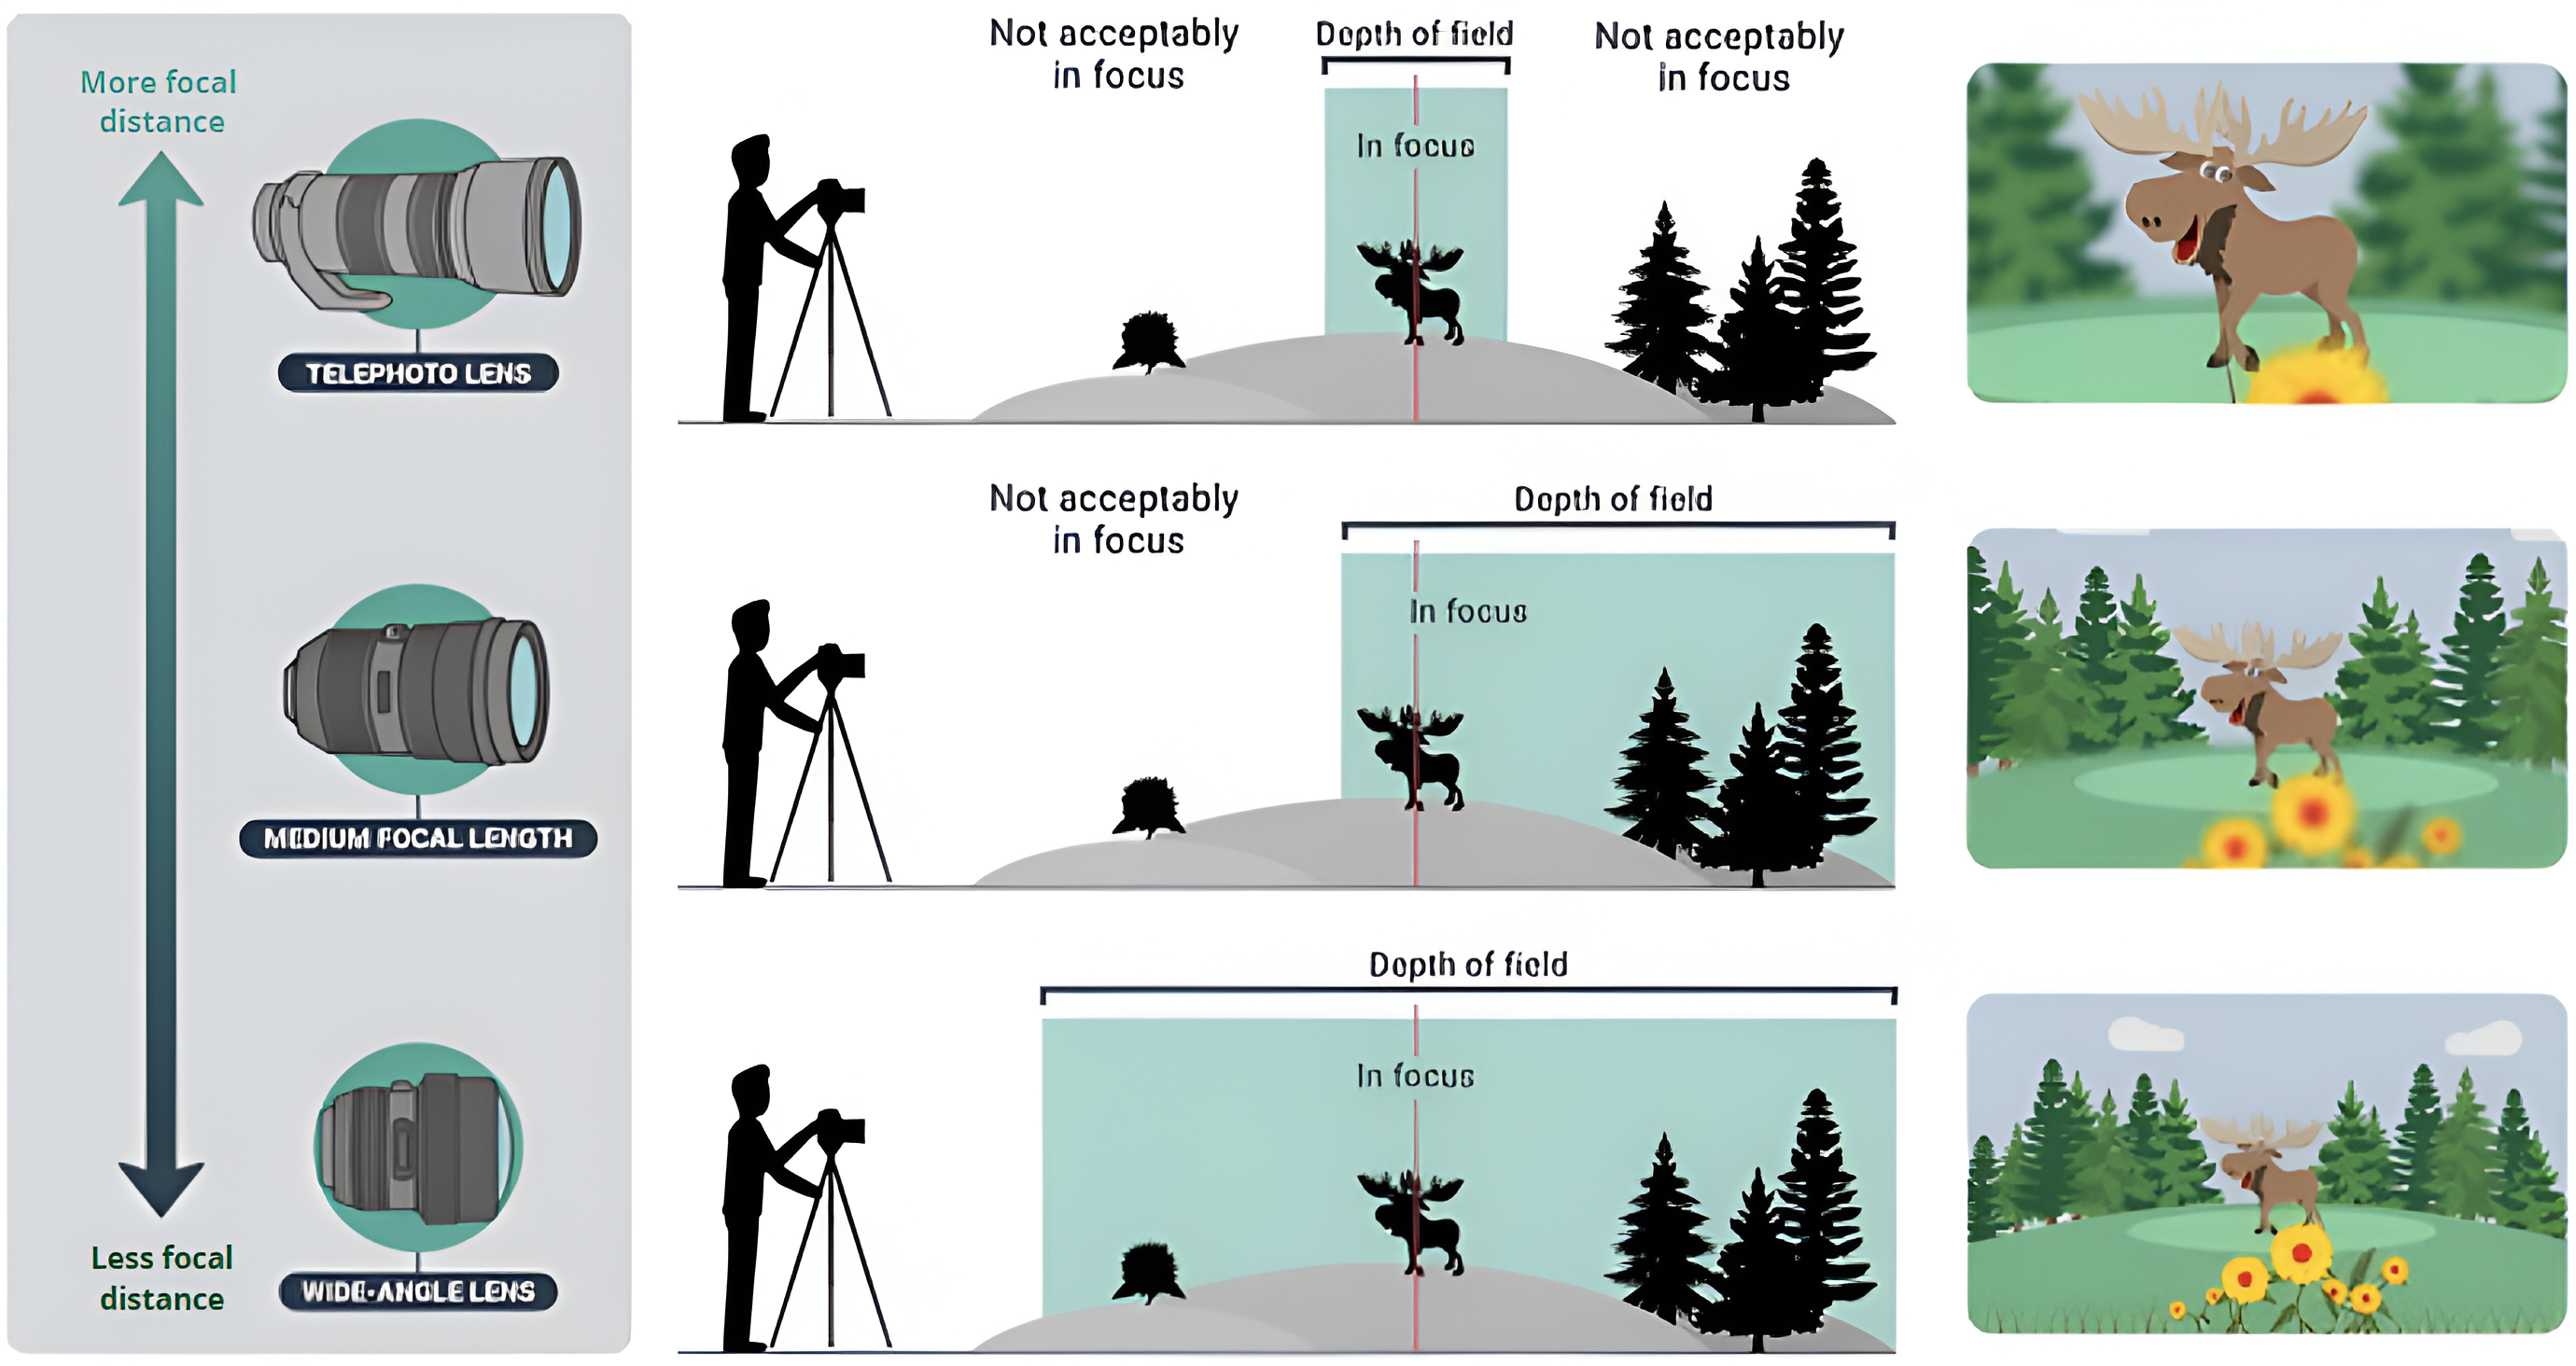
\includegraphics[scale=0.55]{imagenes/cap1/perspective.png}
%	\caption[Relación entre parámetros de la cámara.]{Relación entre longitud focal, distancia cámara-sujeto y profundidad de campo.}
%	\label{fig2.1}
%\end{figure}

En los últimos años se han utilizado varios métodos que combinan técnicas manuales y automatizadas basadas en puntos de referencia o en características anatómicas de la cara\cite{28,30}. Sin embargo, no se han obtenido resultados favorables debido a la dificultad para obtener estimaciones precisas en largas distancias por la diversa fisionomía de la cara, y a los problemas relacionados con los parámetros de la cámara, como el recorte de imágenes o la combinación de diferentes longitudes focales en el mismo conjunto de datos.

Hasta la fecha, uno de los métodos completamente automatizados para estimar la SCD en fotografías faciales es conocido como FacialSCDnet~\cite{14}. Este método emplea una arquitectura basada en aprendizaje profundo para procesar las imágenes faciales y calcular su SCD correspondiente.
Sin embargo, FacialSCDnet presenta ciertas limitaciones. En primer lugar, el conjunto de datos utilizado es limitado, debido al número reducido de individuos y al hecho de que solo incluye adultos. Además, el conjunto de datos sintético empleado para el entrenamiento se limita únicamente a modelos faciales, sin incluir modelos de cuerpo completo. Estos factores aumentan el riesgo de sesgo en el modelo, lo que puede afectar a su capacidad para realizar estimaciones precisas en poblaciones más diversas.

Considerando todos estos aspectos, el presente Trabajo de Fin de Grado (TFG) pretende mejorar el método actual del estado del arte en la estimación automática de la distancia cámara-sujeto en fotografías faciales. Para ello, partimos de FacialSCDnet como una prueba de concepto sólida, reconociendo sus ventajas pero también identificando sus limitaciones inherentes. Nos centraremos en incorporar mejoras significativas que permitan solventar estas limitaciones con el objetivo de elevar el rendimiento y la precisión del sistema.

\section{Motivación}

En el campo del aprendizaje profundo, es común encontrar sesgos en los datos que pueden afectar la precisión y la capacidad de generalización de las soluciones. Estos sesgos pueden surgir debido a varios factores, como la falta de diversidad o el ruido excesivo en el conjunto de datos utilizado para entrenar los modelos. Este fenómeno también se observa en el método FacialSCDnet, el cual fue entrenado con una sola base de datos facial compuesta únicamente por individuos femeninos.
Por lo tanto, para mejorar la calidad del conjunto de datos, sería beneficioso incorporar una mayor diversidad de sujetos en términos de edad, sexo biológico, ascendencia, expresiones faciales, condiciones de iluminación y fondos, así como la inclusión de modelos tanto faciales como de cuerpo completo. 

Una estrategia para abordar este desafío consiste en integrar múltiples bases de datos con el objetivo de construir un conjunto de datos más completo y diverso. Esta mejora contribuiría a una mejor capacidad de generalización y adaptación del modelo, al mitigar los sesgos inherentes a los datos.

Por otro lado, obtener conjuntos de datos reales de alta calidad no siempre es una tarea sencilla. La recopilación y etiquetado de datos pueden resultar costosos y requerir bastante tiempo. En muchos casos, los conjuntos de datos reales disponibles pueden ser limitados en términos de tamaño y diversidad, como ocurre con FacialSCDnet.
Una solución ampliamente utilizada consiste en emplear conjuntos de datos sintéticos en lugar de conjuntos de datos reales \cite{57,58,59}.
El uso de conjuntos de datos sintéticos puede ayudar a reducir costos y tiempo de recopilación de datos, manteniendo o mejorando el rendimiento de los modelos.

Dentro del contexto de FacialSCDnet, una restricción clave reside en la necesidad de conocer la longitud focal y desarrollar un modelo en función de esta. Utilizar imágenes sintéticas, facilita considerablemente la creación de conjuntos de datos según la focal deseada.
Al emplear datos sintéticos, se tiene un mayor control sobre los parámetros de generación, lo que permite ajustar la focal de manera precisa y reproducible.

Con el propósito de aumentar la calidad de los conjuntos de datos empleados en el aprendizaje profundo, particularmente en el contexto de FacialSCDnet, este trabajo se enfoca en reducir sesgos al integrar una mayor diversidad de sujetos y condiciones, además de optimizar los recursos temporales y financieros mediante el uso de conjuntos de datos sintéticos. Este enfoque combinado busca mejorar la capacidad actual de generalización y adaptación de los modelos de FacialSCDnet.

\section{Objetivos}
 El objetivo general de este TFG consiste en desarrollar un mejor modelo de aprendizaje profundo para mejorar la estimación de la distancia cámara-sujeto en fotografías faciales. Para el desarrollo del proyecto, dividiremos el objetivo general en una serie de objetivos parciales:
\begin{enumerate}
    \item Realizar un análisis exhaustivo del estado del arte y de las bases de datos de modelos faciales y humanos 3D.
    \item Desarrollar un protocolo de estandarización y generación de imágenes sintéticas fotorrealistas.
    \item Realizar un estudio comparativo y analizar la viabilidad de la nueva aproximación propuesta.
    \item Explorar el uso de arquitecturas y tecnologías alternativas que permitan mejorar el rendimiento y/o los resultados del método original.
\end{enumerate}

\begin{figure}[h]
	\centering
	\includegraphics[scale=0.35]{imagenes/cap1/resumen.png}
	\caption[Diagrama del proyecto.]{Diagrama del proceso de estimación automática de la SCD en este proyecto.}
	\label{fig3}
\end{figure}

En este contexto, es relevante citar el trabajo de referencia \cite{14}, el cual proporciona una base sólida para el desarrollo del TFG.

\section{Planificación del proyecto}

Para abordar el desarrollo de este proyecto, es esencial considerar que el TFG tiene asignados 12 créditos ECTS, lo que equivale a aproximadamente 300 horas de trabajo. Dada la distribución temporal del segundo cuatrimestre, con unas 20 semanas disponibles, se estima que se requerirá dedicar al TFG unas 20 horas semanales, equivalentes a 4 horas diarias durante 5 días a la semana. Se reservan así 4 semanas como margen para posibles retrasos o imprevistos que puedan surgir durante el desarrollo del proyecto.

En cuanto a la metodología de desarrollo, se ha optado por seguir un enfoque basado en el ciclo de vida en cascada~\cite{38}, aunque con una variante que permite retroalimentación. Aunque el proyecto presenta requisitos y objetivos claros, se reconoce la posibilidad de ajustes menores durante su desarrollo, especialmente a medida que se obtenga más información sobre el problema y los métodos. Esta flexibilidad se considera crucial para adaptarse a posibles cambios en el contexto o los requisitos del proyecto.

A continuación se describen las fases del ciclo de vida del proyecto:
\begin{itemize}
	\item Análisis de Requisitos: Consiste en las reuniones iniciales con los clientes, en este caso los directores del TFG. Se realiza un análisis del problema y un estudio detallado de la bibliografía existente.
	\item Diseño: Consiste en la exploración y selección de los métodos apropiados así como de los conjuntos de datos basados en el análisis previo, tanto para la resolución como para la validación de la solución propuesta. Además, se llevarán a cabo pruebas preliminares y se elaborará el diseño del software experimental.
	\item Implementación: Consiste en la adaptación del código de los modelos investigados, la implementación de nuevas funcionalidades y la generación de un conjunto de datos sintético junto con su posterior preprocesado.
	\item Experimentación: Consiste en la realización de diversos experimentos para validar el funcionamiento del software desarrollado, utilizando los modelos y datos previamente definidos.
	\item Documentación: De forma paralela a las cuatro fases anteriores, se realiza un proceso continuo de documentación de la memoria del proyecto. Este proceso asegura un registro de todas las actividades realizadas, detallando cada paso y decisión tomada durante el desarrollo del proyecto, facilitando así la comprensión y la replicación del trabajo realizado.
\end{itemize}

\begin{table}[h]
	\resizebox{\textwidth}{!}{%
	\begin{tabular}{|c|c|*{4}{c}|*{4}{c}|*{5}{c}|*{4}{c}|*{3}{c}|}
	\hline
	\rowcolor[HTML]{FFC702} 
	\cellcolor[HTML]{FFC702} & \cellcolor[HTML]{FFC702} & \multicolumn{4}{c|}{\cellcolor[HTML]{FFC702}Febrero} & \multicolumn{4}{c|}{\cellcolor[HTML]{FFC702}Marzo} & \multicolumn{5}{c|}{\cellcolor[HTML]{FFC702}Abril} & \multicolumn{4}{c|}{\cellcolor[HTML]{FFC702}Mayo} & \multicolumn{3}{c|}{\cellcolor[HTML]{FFC702}Junio} \\
	\rowcolor[HTML]{FFC702} 
	\multirow{-2}{*}{\cellcolor[HTML]{FFC702}Tarea} & \multirow{-2}{*}{\cellcolor[HTML]{FFC702}\begin{tabular}[c]{@{}c@{}}Semanas\\ - Horas\end{tabular}} & 5 & 12 & 19 & 26 & 4 & 11 & 18 & 25 & 1 & 8 & 15 & 22 & 29 & 6 & 13 & 20 & 27 & 3 & 10 & 17 \\ \hline
	Análisis de Requisitos & 3 - 60 & \cellcolor[HTML]{9B9B9B} & \cellcolor[HTML]{9B9B9B} & \cellcolor[HTML]{9B9B9B} &  &  &  &  &  &  &  &  &  &  &  &  &  &  &  &  &  \\ \cline{1-1}
	Diseño & 3 - 60 &  &  &  & \cellcolor[HTML]{9B9B9B}{\color[HTML]{C0C0C0} } & \cellcolor[HTML]{9B9B9B}{\color[HTML]{C0C0C0} } & \cellcolor[HTML]{9B9B9B}{\color[HTML]{C0C0C0} } &  &  &  &  &  &  &  &  &  &  &  &  &  &  \\ \cline{1-1}
	Implementación & 5 - 90 &  &  &  &  &  &  & \cellcolor[HTML]{9B9B9B} & \cellcolor[HTML]{9B9B9B} & \cellcolor[HTML]{9B9B9B} & \cellcolor[HTML]{9B9B9B} & \cellcolor[HTML]{9B9B9B} &  &  &  &  &  &  &  &  &  \\ \cline{1-1}
	Experimentación & 5 - 90 &  &  &  &  &  &  &  &  &  &  &  & \cellcolor[HTML]{9B9B9B} & \cellcolor[HTML]{9B9B9B} & \cellcolor[HTML]{9B9B9B} & \cellcolor[HTML]{9B9B9B} & \cellcolor[HTML]{9B9B9B} &  &  &  &  \\ \hline
	\end{tabular}%
	}
	\caption{Planificación inicial del proyecto}
	\label{planif-ini}
\end{table}

La planificación inicial se detalla en la tabla \ref{planif-ini}, sin embargo, experimentó varios retrasos, principalmente debido a que el autor también estaba trabajando en un proyecto en colaboración con la Universidad de Granada. Por otro lado, la obtención de los conjuntos de datos 3D no resultó ser una tarea sencilla, debido a su escasa disponibilidad y a los permisos necesarios para acceder a ellos. Además, el preprocesamiento de los datos 3D consumió más tiempo del previsto, ya que, aunque se automatizó en cierta medida, requirió ajustes manuales significativos. Estos contratiempos, junto con el aprendizaje de nuevas librerías por parte del autor, resultaron en modificaciones en la planificación original, tal como se ejemplifica en la tabla \ref{planif-fin}.

\begin{table}[h]
	\centering
	\resizebox{\textwidth}{!}{%
	\begin{tabular}{|c|c|cccc|cccc|ccccc|cccc|ccc|}
	\hline
	\rowcolor[HTML]{FFC702} 
	\cellcolor[HTML]{FFC702} & \cellcolor[HTML]{FFC702} & \multicolumn{4}{c|}{\cellcolor[HTML]{FFC702}Febrero} & \multicolumn{4}{c|}{\cellcolor[HTML]{FFC702}Marzo} & \multicolumn{5}{c|}{\cellcolor[HTML]{FFC702}Abril} & \multicolumn{4}{c|}{\cellcolor[HTML]{FFC702}Mayo} & \multicolumn{3}{c|}{\cellcolor[HTML]{FFC702}Junio} \\
	\rowcolor[HTML]{FFC702} 
	\multirow{-2}{*}{\cellcolor[HTML]{FFC702}Tarea} & \multirow{-2}{*}{\cellcolor[HTML]{FFC702}\begin{tabular}[c]{@{}c@{}}Semanas\\ - Horas\end{tabular}} & 5 & 12 & 19 & 26 & 4 & 11 & 18 & 25 & 1 & 8 & 15 & 22 & 29 & 6 & 13 & 20 & 27 & 3 & 10 & 17 \\ \hline
	Análisis de Requisitos & 3 - 60 & \cellcolor[HTML]{9B9B9B} & \cellcolor[HTML]{9B9B9B} & \cellcolor[HTML]{9B9B9B} &  &  &  &  &  &  &  &  &  &  &  &  &  &  &  &  &  \\ \cline{1-1}
	Diseño & 4 - 70 &  &  &  & \cellcolor[HTML]{9B9B9B}{\color[HTML]{C0C0C0} } & \cellcolor[HTML]{9B9B9B}{\color[HTML]{C0C0C0} } & \cellcolor[HTML]{9B9B9B}{\color[HTML]{C0C0C0} } & \cellcolor[HTML]{9B9B9B} &  &  &  &  &  &  &  &  &  &  &  &  &  \\ \cline{1-1}
	Implementación & 6 - 100 &  &  &  &  &  &  & \cellcolor[HTML]{FFFFFF} & \cellcolor[HTML]{9B9B9B} & \cellcolor[HTML]{9B9B9B} & \cellcolor[HTML]{9B9B9B} & \cellcolor[HTML]{9B9B9B} & \cellcolor[HTML]{FFFFFF} & \cellcolor[HTML]{FFFFFF} & \cellcolor[HTML]{9B9B9B} & \cellcolor[HTML]{9B9B9B} &  &  &  &  &  \\ \cline{1-1}
	Experimentación & 6 - 100 &  &  &  &  &  &  &  &  &  & \cellcolor[HTML]{FFFFFF}{\color[HTML]{FFFFFF} } & \cellcolor[HTML]{FFFFFF}{\color[HTML]{FFFFFF} } & \cellcolor[HTML]{9B9B9B}{\color[HTML]{9B9B9B} } & \cellcolor[HTML]{9B9B9B}{\color[HTML]{9B9B9B} } & \cellcolor[HTML]{FFFFFF} & \cellcolor[HTML]{FFFFFF} & \cellcolor[HTML]{9B9B9B} & \cellcolor[HTML]{9B9B9B} & \cellcolor[HTML]{9B9B9B} & \cellcolor[HTML]{9B9B9B} &  \\ \hline
	\end{tabular}%
	}
	\caption{Planificación final del proyecto}
	\label{planif-fin}
\end{table}

% Aquí las dimensiones económicas

Para estimar los costos, comenzamos considerando un salario de 30 euros por hora para un responsable I+D en una empresa tecnológica o para un investigador senior. Además de esto, se contemplan los gastos asociados a los materiales, como el costo del portátil utilizado en el desarrollo del TFG y el uso de un servidor GPU de alto rendimiento. Estos costes se desglosan detalladamente en la Tabla \ref{tab:coste-proyecto}. 

En relación al servidor GPU, su valoración se estima en x euros...

[Aún no sé qué día se va a terminar así que no puedo calcular la duración ni el salario, y respecto al servidor no entiendo muy bien lo de las amortizaciones]

\begin{table}[h]
	\centering
	\begin{tabular}{ll}
	\hline
	\multicolumn{1}{|l|}{\cellcolor[HTML]{FFCB2F}Fecha de inicio} & \multicolumn{1}{l|}{05/02/2024} \\ \hline
	\multicolumn{1}{|l|}{\cellcolor[HTML]{FFCB2F}Fecha de fin} & \multicolumn{1}{l|}{} \\ \hline
	\multicolumn{1}{|l|}{\cellcolor[HTML]{FFCB2F}Duración} & \multicolumn{1}{l|}{} \\ \hline
	 &  \\ \hline
	\rowcolor[HTML]{FFCB2F} 
	\multicolumn{1}{|l|}{\cellcolor[HTML]{FFCB2F}Item} & \multicolumn{1}{l|}{\cellcolor[HTML]{FFCB2F}Costo} \\ \hline
	\multicolumn{1}{|l|}{Salario} & \multicolumn{1}{l|}{} \\ \hline
	\multicolumn{1}{|l|}{Portátil de Gama Alta} & \multicolumn{1}{l|}{2.600 euros} \\ \hline
	\multicolumn{1}{|l|}{Servidor GPU} & \multicolumn{1}{l|}{} \\ \hline
	\multicolumn{1}{|l|}{\cellcolor[HTML]{FFCB2F}Total} & \multicolumn{1}{l|}{} \\ \hline
	\end{tabular}
	\caption{Estimación del coste del proyecto}
	\label{tab:coste-proyecto}
\end{table}